%! TEX root = ../000-main.tex
\chapter{Nonlinear dimensionality reduction}
\chaptermark{NL dim. red.}

\section[Introduction]{Introduction to dimensionality reduction}
\paragraph{References:}
\cite[Chapter 8]{johnson_applied_2007},
\cite[Chapters 5 and 6]{pena_alisis_2002},
\cite[Section 11.1]{venables_exploratory_2002},
\cite[Sections 14.5.1, 14.8 and 14.9]{hastie_elements_2009}

We observe $n$ independent objects $\mathcal{O}_i,\;i=1,\ldots,n$ from a given population.

In general, they belong to a large-dimensional (or even infinite-dimensional) space $\Omega$.

\begin{problem}{Dimensionality reduction problem}{}
We want to find a low dimensional configuration $\boldsymbol{Y}$, that is an
$n \times q$ matrix, where $q < n$ such that each of its rows $\boldsymbol{y}_i$ can
be identified with the observed object $\mathcal{O}_i$ in some way:
\begin{itemize}
	\item An application $\rho: \mathbb{R}^q \to \Omega$ such that
	      $\rho(\boldsymbol{y}_i) \approxeq \mathcal{O}_i,\quad i=1,\ldots,n$.
	\item We can define a distance between $\boldsymbol{y}_i$ and $\boldsymbol{y}_j$,
	      such that the distance between $\mathcal{O}_i$ and $\mathcal{O}_j$ is close
	      to the dissimilarity between the observed objects $\mathcal{O}_i$ and
	      $\mathcal{O}_j,\; \forall i,j \in \{1,\ldots,n\}$.
	\item \ldots
\end{itemize}
\begin{note}
	When dimensionality reduction is for visualization purposes, $q = 2$ is
	usually chosen.
\end{note}
\end{problem}

\subsection{Two types of information from the observed objects}
We consider two different ways of extracting information from the observed objects:
\begin{itemize}
	\item Sampling information as a \iemph{data matrix} $\boldsymbol{X}$ of
	      size $n \times p$ ($n$ individuals and $p$ attributes, $p \gg q$).
	      \begin{itemize}
		      \item Principal component analysis (PCA).
		      \item Principal curves (Nonlinear version of PCA) \cite{hastie_principal_1989,delicado_another_2001}.
	      \end{itemize}
	\item Sampling information as a distance matrix $\boldsymbol{D}$ of size
	      $n \times n$.
	      \begin{itemize}
		      \item Multidimensional scaling (MDS).
		      \item Local MDS
		      \item Isometric mapping (ISOMAP, Nonlinear version of MDS).
		      \item t-Stochastic Neighbor Embedding (t-SNE).
	      \end{itemize}
\end{itemize}

\section[Principal Component Analysis]{Principal Component Analysis (PCA)}\index{PCA}

\begin{definition}{Principal component analysis (PCA)}{PCA}
	Multivariate analysis technique that intends to explain the
	\iemph{variance-covariance structure} through a few linear combinations of the original
	variables.

	\paragraph{Main goals:} Interpretation and dimensionality reduction.
\end{definition}

\begin{definition}{Variance-covariance structure}{}
	The variance-covariance structure of a random vector $\boldsymbol{X} \in \mathbb{R}^p$
	is defined as the $p \times p$ matrix $\boldsymbol{V} = \boldsymbol{V}(\boldsymbol{X})$
	such that:
	\begin{equation*}
		\boldsymbol{V}_{ij} = \mathrm{Cov}(X_i,X_j) = \mathrm{E}[(X_i - \mathrm{E}[X_i])(X_j - \mathrm{E}[X_j])].
	\end{equation*}
	\tcblower
	The variance is the diagonal of the variance-covariance matrix:
	\begin{equation*}
		\boldsymbol{\sigma}^2 = \mathrm{diag}(\boldsymbol{V}).
	\end{equation*}
\end{definition}

\subsubsection{Finding the first principal component (q=1)}
\begin{figure}[H]
	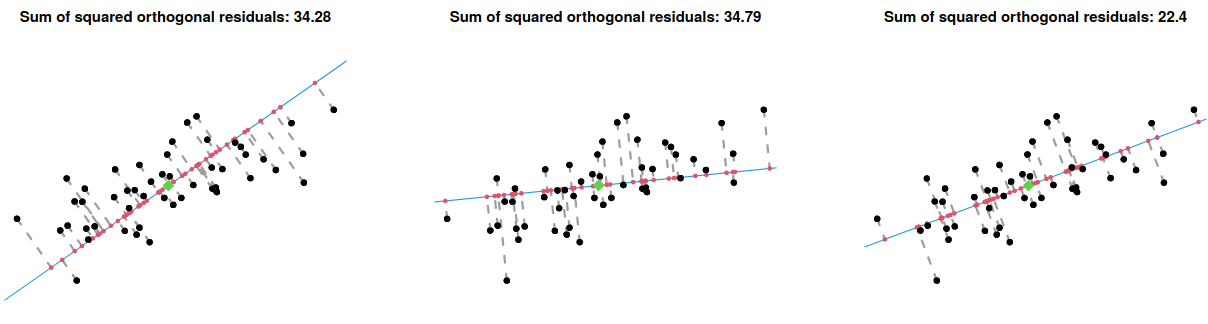
\includegraphics{pca_q1}
\end{figure}
We observe $\boldsymbol{x}_i \in \mathbb{R}^p,\;i=1,\ldots,n$ with mean $\boldsymbol{m}$.
For $\boldsymbol{a} \in \mathbb{R}^p,\, \lVert \boldsymbol a \rVert = 1$, the
projection vector of $(\boldsymbol{x} - \boldsymbol{m})$ in the direction of $\boldsymbol{a}$ is:
$P_{\boldsymbol{a}}(\boldsymbol{x} - \boldsymbol{m}) = \bigl( (\boldsymbol x - \boldsymbol m)' \boldsymbol a \bigr)
	\boldsymbol{a}$. These two problems:
\begin{align*}
	\min_{\boldsymbol{a} \in \mathbb{R}^p,\, \lVert \boldsymbol a \rVert = 1} & \sum_{i=1}^n
	\left\lVert \boldsymbol{x}_i - \boldsymbol{m} - P_{\boldsymbol{a}}(\boldsymbol{x}_i - \boldsymbol{m}) \right\rVert^2 \tag{Minimizing the orthogonal residuals} \\
	\max_{\boldsymbol{a} \in \mathbb{R}^p,\, \lVert \boldsymbol a \rVert = 1} & \sum_{i=1}^n
	\left\lVert P_{\boldsymbol{a}}(\boldsymbol{x}_i - \boldsymbol{m}) \right\rVert^2
	\tag{Maximizing the inertia of the projected data}
\end{align*}
have the same solution $\boldsymbol{a}^*$, which we will call the \iemph{first principal component},
by Pythagoras' theorem:
\begin{equation*}
	\sum_{i=1}^n \left\lVert \boldsymbol{x}_i - \boldsymbol{m} \right\rVert^2
	= \sum_{i=1}^n \left\lVert
	\boldsymbol{x}_i - \boldsymbol{m} - P_{\boldsymbol{a}^*}(\boldsymbol{x}_i - \boldsymbol{m})
	\right\rVert^2
	+ \sum_{i=1}^n \left\lVert P_{\boldsymbol{a}^*}(\boldsymbol{x}_i - \boldsymbol{m}) \right\rVert^2.
\end{equation*}

Let $\hat{V} = (\boldsymbol{v}_1,\ldots,\boldsymbol{v}_p)$ and $\hat{D} = \mathrm{Diag}(\hat{\lambda}_1,\ldots,\hat{\lambda}_p)$

Let $\boldsymbol S = \hat{V}\hat{D}\hat{V}'$ be the spectral decomposition of $\boldsymbol{S}$.

Then, the data matrix of sampling principal components is:
\begin{equation*}
	\boldsymbol{Y} = (\boldsymbol{y}_1,\ldots,\boldsymbol{y}_n) = (\boldsymbol{X} - \boldsymbol 1_n \boldsymbol m ')\hat{V}.
\end{equation*}
Roughly speaking, the sampling principal components are uncorrelated linear combinations of the
observed variables having the largest possible variability.

\begin{note}
	In this, way one of the two main goals of PCA is met: Interpretation.
\end{note}

\subsection{Single value decomposition (SVD)}

\begin{theorem}{Singular-Value Decomposition}{svd}
	Let $A$ be an $n \times p$ matrix. Then there exists an orthogonal matrix $U$ of size $n \times n$,
	and a orthogonal matrix $V$ of size $p \times p$ such that:
	\begin{equation*}
		A = U \Gamma V'
	\end{equation*}
	Where the $n \times p$ matrix $\Gamma$ has $(i,\, i)$ entry $\gamma_i \geq 0,\;i=1,\ldots,\min(n,p)$
	and the other entries are zero (diagonal matrix). The positive entries $\gamma_i$ are called
	the \iemph{singular values} of $A$. The number of singular values coincides with $k$, the rank of $A$.
	\tcblower
	\paragraph{Remark:} Let $\boldsymbol{u}_i$ be the columns of $U$ and let $\boldsymbol{v}_i'$ be the
	rows of $V'$. Then:
	\begin{equation*}
		A = U \Gamma V' = \sum_{i=1}^k \gamma_i \boldsymbol{u}_i \boldsymbol{v}_i'
	\end{equation*}
\end{theorem}

\subsubsection{SVD and PCA}

Let $A = \boldsymbol{X} - \boldsymbol 1_n \boldsymbol m '$. Then $A'A = (n - 1) \boldsymbol{S} =
	(n - 1) \hat{V} \hat{D} \hat{V}'$.

Let $(\boldsymbol X - \boldsymbol 1_n \boldsymbol m ') = \hat{U}\Gamma \hat{V}'$ be SVD of $A$

$\boldsymbol{Y} = (\boldsymbol X - \boldsymbol 1_n \boldsymbol m ') \hat{V} \iff
	\boldsymbol Y \hat{V}' = (\boldsymbol X - \boldsymbol 1_n \boldsymbol m ') = \hat{U}\Gamma\hat{V}'$,
then $\boldsymbol{Y} = \hat{U}\Gamma$.

The best approximation of rank $s$ to $A$ is:
\begin{equation*}
	\sum_{j=1}^s \gamma_j \boldsymbol{u}_j \boldsymbol{v}_j' = \sum_{j=1}^s \boldsymbol{y}_j \boldsymbol{v}_j'
\end{equation*}
Therefore, the best approximation to $\boldsymbol{X}$ of rank $s$ is:
\begin{equation*}
	\boldsymbol{X} \approx \boldsymbol 1_n \boldsymbol m ' + \sum_{j=1}^s \boldsymbol{y}_j \boldsymbol{v}_j'
\end{equation*}
For the $i$-th row of $\boldsymbol{X}$:
\begin{equation*}
	\boldsymbol{x}_i \approx \boldsymbol{m} + \sum_{j=1}^s y_{ij} \boldsymbol{v}_j'
\end{equation*}
where $y_{ij}$ is the score of the $i$-th observation on the $j$-th principal component.

\begin{note}
	With this, the second goal of PCA is met: Dimensionality reduction.
\end{note}

\section{Multidimensional scaling (MDS)}

\begin{definition}{Multidimensional scaling (MDS)}{mds}\index{mds}
	is a dimensionality reduction technique based on \emph{inter-individual distances}.
\end{definition}

\begin{definition}{Euclidean configuration}{}
	For $n$ individuals, let $\boldsymbol{D} = (\delta_{ij})$ be the $n \times n$ matrix of inter-individual
	distances.

	Assume that for a $q \leq n$ there exists a $n \times q$ data matrix $\boldsymbol{X}$ such that
	the Euclidean distance between the $i$-th and $j$-th row of $\boldsymbol{X}$,
	$\left\lVert \boldsymbol{x}_i - \boldsymbol{x}_j \right\rVert$, is equal to $\delta_{ij}$.

	We say that $\boldsymbol{X}$ is a \iemph{Euclidean configuration} of $\boldsymbol{D}$.
	\tcblower
	\begin{note}
		Such configuration does not always exist.
	\end{note}
\end{definition}

\begin{definition}{Principal coordinates}
When it does exist, $\boldsymbol{D}$ is said to be Euclidean. In this
case $\boldsymbol{X}$ can be chosen verifying the following conditions:
\begin{itemize}
	\item It has orthogonal columns.
	\item For $1 \leq q \leq r$, the first $q$ columns of $\boldsymbol{X}$,
	      $\boldsymbol{\tilde{X}}_a$, make up the $q$-dimensional configuration that
	      best approximates the observed distances.
\end{itemize}
The columns of $\boldsymbol{X}$ are called \iemph{principal coordinates}.

\tcblower

\begin{note}
When an Euclidean configuration does not exist, MDS allows to
obtain \emph{approximated solution}s.

That is, MDS looks for a $q$-dimensional
configuration $\boldsymbol{X}$ such that the Euclidean distances between
the rows of $\boldsymbol{X}$ are \emph{as close as possible} to the observed
distances.
\end{note}
\end{definition}


\subsection{Classical metric scaling}

If a $n \times p$ matrix $\boldsymbol{X}$ (with 0 mean by columns) is observed
and Euclidean distances are used, then: \emph{MDS and PCA give the same results}.

\subsection{Non-classical metric scaling}%
\label{sec:non-classical-metric-scaling}

Let $\boldsymbol{D} = (\delta_{ij})^n_{i,j=1}$ be the inter-individual distance
matrix recorded for the $n$ objects forming our sample.

Fix a tentative dimension $q$ and a $n \times q$ matrix $\boldsymbol{X}$.
Let $d_{ij} = \left\lVert \boldsymbol{x}_i - \boldsymbol{x}_j \right\rVert$ be the
Euclidean distance between the $i$-th and $j$-th row of $\boldsymbol{X}$.

The metric \iemph{STRESS} (STandardized REsidual Sum of Squares), a measure
of the relative error made when matrix $\boldsymbol{X}$ is considered as
an Euclidean configuration for the distance matrix $\boldsymbol{D}$, is defined as:
\begin{equation*}
	\text{STRESS}_M(\boldsymbol{D}, \boldsymbol{X}) = \sqrt{\frac
		{\sum_{i<j}(\delta_{ij} - d_{ij})^2}
		{\sum_{i<j}\delta_{ij}^2}
	}
\end{equation*}

\begin{problem}{Non-classical metric scaling}{}
\begin{equation*}
	\min_{\boldsymbol{X} \in \mathds{R}^{n\times q}} \text{STRESS}_M(\boldsymbol{D}, \boldsymbol{X})
\end{equation*}
\end{problem}

There is also S-STRESS:
\begin{equation*}
	\text{S-STRESS}_M(\boldsymbol{D}, \boldsymbol{X}) = \sqrt{\frac
		{\sum_{i<j}(\delta_{ij}^2 - d_{ij}^2)^2}
		{\sum_{i<j}\delta_{ij}^4}
	}
\end{equation*}

\subsection{Non-metric scaling}
Non-metric scaling uses only the ranks of the inter-individual distances $\delta_{ij}$.
The metric used is the Non-metric Stress (NMS):
\begin{equation*}
	\text{STRESS}_{NM}(\boldsymbol{D}, \boldsymbol{X}, f) = \sqrt{\frac
	{\sum_{i<j}(\text{rank}(\delta_{ij}) - d_{ij})^2}
	{\sum_{i<j}d_{ij}^2}
	}
\end{equation*}
Where $f: \mathds{R}^+ \to \mathds{R}^+$ is an increasing function.

\begin{problem}{Non-metric scaling}{}
\begin{equation*}
	\min_{\boldsymbol{X} \in \mathds{R}^{n\times q}} \min_{f\uparrow} \text{STRESS}_{NM}(\boldsymbol{D}, \boldsymbol{X}, f)
\end{equation*}
\end{problem}

\section{Distances and similarities}

\begin{definition}{Metric and Semi-metric}{metric}

	Let $\Omega$ be a set of objects. The application:
	\begin{equation*}
		d: \Omega \times \Omega \to \mathds{R}
	\end{equation*}
	is a \iemph{semi-metric} if it verifies the following properties $\forall P, Q, R \in \Omega$:
	\begin{align*}
		d(P, Q) & = d(Q, P) \tag{symmetry}                         \\
		d(P, Q) & \geq 0 \tag{non-negativity}                      \\
		d(P, P) & = 0 \tag{identity}                               \\
		d(P, Q) & \leq d(P, R) + d(R, Q) \tag{triangle inequality}
	\end{align*}

	\begin{marker}
		Additionally, if $d(P, Q) = 0 \implies P = Q$, then $d$ is a \iemph{metric} (or \emph{distance}).
	\end{marker}
\end{definition}

\begin{definition}{Similarity}{similarity}

	Let $\Omega$ be a set of objects. The application:
	\begin{equation*}
		s: \Omega \times \Omega \to \mathds{R}
	\end{equation*}
	is a \iemph{similarity} if it verifies the following properties $\forall P, Q, R \in \Omega$:
	\begin{align*}
		s(P, Q) & = s(Q, P) \tag{symmetry}    \\
		s(P, Q) & \geq 0 \tag{non-negativity} \\
		s(P, P) & = s(Q, Q)                   \\
		s(P, Q) & \leq s(R, R)
	\end{align*}
	Additionally, it is required that $s(P, Q)$ is an increasing function of
	the proximity between $P$ and $Q$.
\end{definition}

\subsection{Similarities to and from distances}
\begin{equation*}
	s(P, Q) = \frac{1}{1 + d(P, Q)}
\end{equation*}

If the similarity function $s$ is a valid kernel function with $s(P, P) = 1,\;\forall P\in\Omega$,
and $s(P, Q) < 1,\;\forall P \neq Q \in \Omega$, then:
\begin{equation*}
	d(P, Q) = \sqrt{2\bigl(1 - s(P, Q)\bigr)}
\end{equation*}

\pagebreak
\section{Principal Curves}

\subsection{Introduction}

\begin{definition}{First principal component}{}
	The straight line fitting best a data cloud.
\end{definition}

\begin{problem}{Principal curves}{}
Given a dataset with a non-elliptical configuration,
look for the curve best fitting the data.
\end{problem}

\begin{definition}{Principal curves}{}
	Smooth one-dimensional curves that pass through the middle of a
	$p$-dimensional data set, providing a non-linear summary of the data.
	\cite{hastie_principal_1989}
	\tcblower
	\begin{note}
		Principal curves are \emph{non-linear} and \emph{non-parametric} generalizations
		of the first principal component.
	\end{note}
\end{definition}

\subsection{Dimensionality reduction by a curve}
We observe $n$ independent objects $\mathcal{O}_i = \boldsymbol{x}_i,\, i = 1, \dots, n$ from
a r.v.%
\footnote{Random variable}
$\boldsymbol{X}$ with values in the large dimensional space $\Omega = \mathds{R}^p$.
\begin{problem}{Dimensionality reduction by a curve}{}
Looking for a \emph{one-dimensional} configuration $\boldsymbol{y} \in \mathds{R}^n$ such
that each value $y_i$ of $\boldsymbol{y}$ can be identified with the observed
$\boldsymbol{x}_i$ in the following way:

There exists a one-dimensional differentiable parametric function $\alpha$ from
$[a, b] \subseteq \mathds{R} \to \mathds{R}^p$ whose image:
\begin{equation*}
	\left\{ \boldsymbol{x} \in \mathds{R}^p \mid \boldsymbol{x} = \alpha(y), \, y \in [a, b]  \right\}
\end{equation*}
is called a \iemph{curve}, such that $\alpha(y_i)$ is close to the observed $\boldsymbol{x}_i$ for
all $i = 1, \dots, n$.
\tcblower
\begin{note}
	The function $\alpha : \mathds{R} \to \mathds{R}^p$ is also called a \emph{curve}.
\end{note}
\begin{note}
	For dimension $q$, $1 < q < p$, the concept of \iemph{manifold} $\rho: \mathds{R}^q \to \mathds{R}^p$
	extends that of curve to a $q$-dimensional space.
\end{note}
\end{problem}

\subsection{Principal curves according to Hastie and Stuetzle}

The first definition of principal curves was given by Hastie and Stuetzle in \cite{hastie_principal_1989}.
It does not include parametric assumptions.

The definition is based on the concept of \emph{self-consistency}:
\begin{definition}{HSPC}{}
	A curve $\alpha$ is a \iemph{Hastie-Stuetzle principal curve} if it is self-consistent.
\end{definition}

\begin{definition}{Self-consistency (curves)}{}
	A curve $\alpha$ is \iemph{self-consistent} if for all $\alpha(s)$ in the curve,
	this point is the conditional mean of $\boldsymbol X$ given that $\boldsymbol X$ belongs
	to the attraction domain of $\alpha(s)$.
\end{definition}

\begin{definition}{Domain of attraction of a point of $\alpha(s)$}{}

	The domain of attraction of a point $\alpha(s)$ in a differentiable curve $\alpha$
	is, usually, the orthogonal hyperplane to $\alpha$ at $\alpha(s)$:
	\begin{equation*}
		H(\alpha(s), \alpha'(s)) = \left\{
		\boldsymbol{y} \in \mathds{R}^p \mid \boldsymbol{y} - \alpha(s) \perp \alpha'(s)
		\right\}
	\end{equation*}
	Where $\alpha'(s)$ is the \iemph{velocity vector} to $\alpha$ at $s$, which is
	the component-wise derivative of $\alpha$ and it is tangent to $\alpha$ at $\alpha(s)$.
\end{definition}

\begin{figure}[H]
	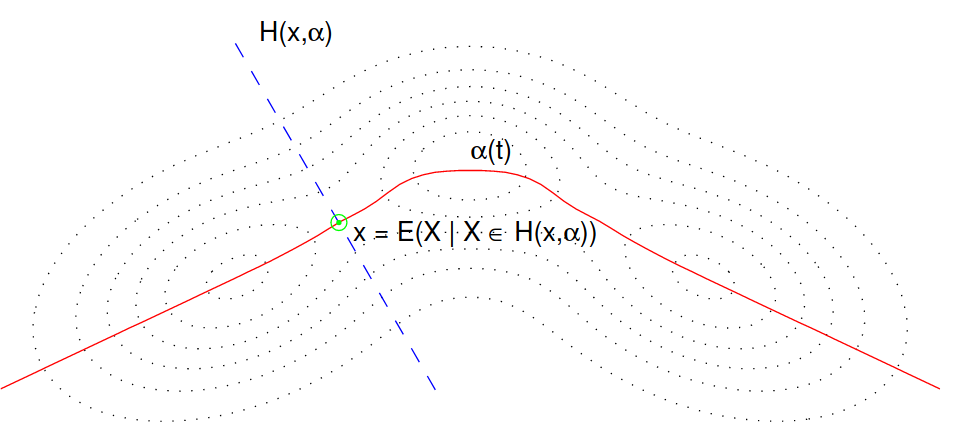
\includegraphics{hspc}
	\caption{Hastie-Stuetzle principal curve}
\end{figure}

\subsubsection{Theoretical drawbacks of HSPCs}

\begin{itemize}
	\item Neither existence nor uniqueness of HSPCs is guaranteed.
	\item Let $S$ be a r.v. in $\mathds{R}$, let $\alpha: \mathds{R} \to \mathds{R}^p$, let $\varepsilon$
	      be a zero-mean r.v. in $\mathds{R}^p$, $S$ and $\varepsilon$ are independent. Define
	      $\boldsymbol{X} = \alpha(S) + \varepsilon$. Then, in general, the
	      generating curve $\alpha$ is not a HSPC of $\boldsymbol{X}$.
	\item For a $p$-dimensional normal distribution, all the principal components are HSPC. Which
	      means that HSPC are generalizing a property that does not characterize uniquely the first
	      principal component.
\end{itemize}

\subsubsection{Theoretical algorithm for HSPC}

The algorithm proposed by Hastie and Stutzle to find the principal curve
consists of the iteration until convergence of the function $\mathcal W_{\boldsymbol X}$:
\begin{equation*}
	\alpha_{k+1} = \mathcal W_{\boldsymbol X}(\alpha_k) =
	\left\{
	\boldsymbol x \in \mathds{R}^p : \boldsymbol x = \mathds{E}(\boldsymbol X \mid \boldsymbol X \in
	D_{\alpha_k}(\boldsymbol y)) \mid \text{for some }\boldsymbol y \in \alpha_k
	\right\}
\end{equation*}
that is, for any $s \in [a, b] \subseteq \mathds{R}$:
\begin{equation*}
	\alpha_{k+1}(s) = \mathds{E}(\boldsymbol X \mid \boldsymbol X \in H(\alpha_k(s), \alpha_k'(s)))
\end{equation*}
with the first principal component (PC1) line as initial set $\alpha_0$.

\paragraph{Practical computation}
In practice, populational concepts are replaced by sampling ones:
\begin{itemize}
	\item PC1 is replaced by the set of the projected observed points on the line:
	      \begin{equation*}
		      \alpha_0 = \left\{
		      \boldsymbol y_i = \boldsymbol{\overline{x}}_n + s_i \boldsymbol{v}_1 \mid i = 1, \dots, n
		      \right\}
	      \end{equation*}
	      Where $\boldsymbol{\overline{x}}_n$ is the sample mean of the observed points and, $\boldsymbol{v}_1$
	      is the direction of the first principal component and $s_i$ are the scores of the observed
	      data on PC1.
	\item Numerical derivation is used to compute the velocity vector $\alpha_k'(s_i)$.
	\item Smoothing methods are used to estimate the conditional expectations
	      $\mathds{E}(\boldsymbol X \mid \boldsymbol X \in H(\alpha_k(s), \alpha_k'(s)))$.
\end{itemize}
\begin{note}
	The algorithm that computes HSPC is implemented in the \texttt{princurve} package in R.
\end{note}

\subsection{Principal curves of oriented points}

Delicado \cite{delicado_another_2001} propeses to generalize the following property of the
first principal component (the straight line
$\{\mathds{E}(\boldsymbol X) + s \boldsymbol v_1 \mid s \in \mathds{R}\}$)
in a multivariate normal random variable $\boldsymbol X$:
\begin{equation*}
	TV(\boldsymbol X \mid \boldsymbol X \in H(\boldsymbol x, \boldsymbol v_1))
	\leq
	TV(\boldsymbol X \mid \boldsymbol X \in H(\boldsymbol x, \boldsymbol b))
\end{equation*}
for any direction $\boldsymbol b \in S^{p-1}$ and any point $\boldsymbol x \in \mathds{R}^p$,
where $H(\boldsymbol x, \boldsymbol b) = \left\{
	\boldsymbol y \in \mathds{R}^p \mid \boldsymbol y - \boldsymbol x \perp \boldsymbol b
	\right\}$
is the hyperplane orthogonal to $\boldsymbol b$ at $\boldsymbol x$.
$TV$ denotes the \iemph{Total Variance}.

Moreover, the point $\mathds{E}(\boldsymbol X \mid \boldsymbol X \in H(\boldsymbol x, \boldsymbol b))$
is located over the first component of $\boldsymbol X$ for all $\boldsymbol x \in \mathds{R}^p$.

\subsubsection{Some definitions}

Let $\boldsymbol X$ be a $p$-dimensional r.v. with density $f$ and finite
second order moments.

Let $\boldsymbol b \in S^{p-1} = \{\boldsymbol w \in \mathds{R}^p \mid
	\lVert \boldsymbol w \rVert = 1\}$ and $\boldsymbol x \in \mathds{R}^p$.

$H(\boldsymbol x, \boldsymbol b) = \left\{
	\boldsymbol y \in \mathds{R}^p \mid \boldsymbol y - \boldsymbol x \perp \boldsymbol b
	\right\}$ is the hyperplane orthogonal to $\boldsymbol b$ at $\boldsymbol x$.

$TV(\boldsymbol Y) = \text{Trace}(V(\boldsymbol Y))$ is the Total Variance of $\boldsymbol Y$.

We say that $\alpha : \mathds{R} \to \mathds{R}^p$ is \iemph{parameterized by the arch length}
if the curve length from $\alpha(s_1)$ to $\alpha(s_2)$ is equal to $|s_2 - s_1|$.

It is also said that $\alpha$ is \iemph{unit speed parameterized} if $\lVert \alpha'(s) \rVert = 1,\,\forall s$.
\begin{align*}
	\mu(\boldsymbol x, \boldsymbol b)  & = \mathds{E}(\boldsymbol X \mid \boldsymbol X \in H(\boldsymbol x, \boldsymbol b)) \\
	\phi(\boldsymbol x, \boldsymbol b) & = TV(\boldsymbol X \mid \boldsymbol X \in H(\boldsymbol x, \boldsymbol b))
\end{align*}
\begin{alignat*}{2}
	\boldsymbol b^*   & : \mathds{R}^p \to S^{p-1}      & \quad \boldsymbol b^*(\boldsymbol x)   & = \argmin_{\boldsymbol b \in S^{p-1}} \phi(\boldsymbol x, \boldsymbol b) \\
	\boldsymbol \mu^* & : \mathds{R}^p \to \mathds{R}^p & \quad \boldsymbol \mu^*(\boldsymbol x) & = \boldsymbol \mu(\boldsymbol x, \boldsymbol b^*(\boldsymbol x))         \\
	\phi^*            & : \mathds{R}^p \to \mathds{R}   & \quad \phi^*(\boldsymbol x)            & = \phi(\boldsymbol x, \boldsymbol b^*(\boldsymbol x))
\end{alignat*}
We say that $\boldsymbol b^*(\boldsymbol x)$ is the \iemph{principal direction} of $\boldsymbol x$.

The smoothness of the functions $\mu, \phi, \boldsymbol b^*, \boldsymbol \mu^*$ and $\phi^*$ depend
on the smoothness of the density function $f$ of $\boldsymbol X$.

\begin{figure}[H]
	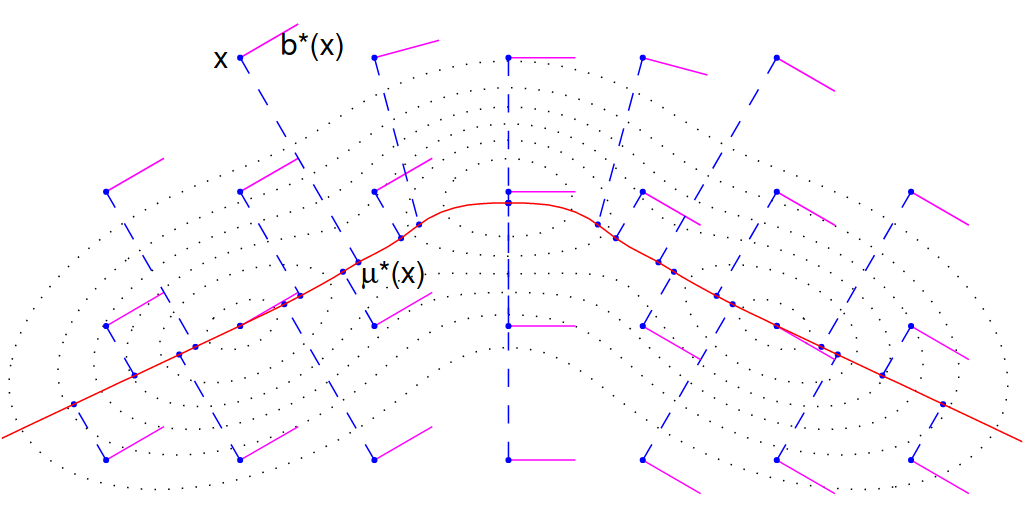
\includegraphics{deli}
	\caption{Illustration of the principal direction of a point $\boldsymbol x$}
\end{figure}

\subsubsection{Multivariate normal case}
\begin{prop}{}{}
	Let $\boldsymbol X \sim N_p(\mu, \Sigma)$. Let $\lambda_1$ be the largest eigenvalue of $\Sigma$
	and let $\boldsymbol v_1$ be the corresponding unit norm eigenvector.

	The following properties hold:
	\begin{enumerate}
		\item For all $\boldsymbol x \in \mathds{R}^p$, the correspondence $\boldsymbol b^*$ is in
		      fact a function and: $\boldsymbol b^*(\boldsymbol x_0) = \boldsymbol v_1,\,\forall\boldsymbol x_0$.
		\item For all $\boldsymbol x \in \mathds{R}^p$, the point $\boldsymbol x_1 = \mu^*(\boldsymbol x_0)$
		      belongs to the straight line defined by the first principal component:
		      $\{\mu + s\boldsymbol v_1 \mid s \in \mathds R\}$
		\item A point $\boldsymbol x \in \mathds{R}^p$ belongs to the first principal component
		      straight line if and only if $\boldsymbol x_1$ is a fixed point of the function
		      $\boldsymbol \mu^*$, that is if and only if $\boldsymbol x_1 = \boldsymbol \mu^*(\boldsymbol x_1)$.
	\end{enumerate}
\end{prop}

Only \emph{local information} around the hyperplane $H(\boldsymbol x, \boldsymbol v)$ is required
to check whether or not the pair $(\boldsymbol x, \boldsymbol v)$ identifies the first principal
component.

A mechanism to find points in the first principal component iterating the function
$\mu^*$ we arrive (in just on step) from any point
$\boldsymbol x_0$ to a point $\boldsymbol x_1$ in the first principal component.

The idea of looking for points $\boldsymbol x$ that are fixed points of the application
$\boldsymbol \mu^*$ easily generalizes when the v.a. $\boldsymbol X$ does not have a normal
distribution.

\begin{definition}{Principal oriented points (POP)}{}\index{POP}\index{principal oriented points}
	The set of fixed points of $\boldsymbol \mu^*$:
	\begin{equation*}
		\Gamma(\boldsymbol X) = \left\{
		\boldsymbol x \in \mathds{R}^p \mid \boldsymbol x = \boldsymbol \mu^*(\boldsymbol x)
		\right\}
	\end{equation*}
\end{definition}

\begin{definition}{Principal curve of oriented points (PCOP)}{}

	Let $\alpha : \mathds{R} \to \mathds{R}^p$ be a continuous curve parameterized by the arc length.
	We say that $\alpha$ is a \iemph{principal curve of oriented points} for $\boldsymbol X$ if:
	\begin{equation*}
		\{
		\alpha(s) \mid s \in [a, b]
		\} \subseteq \Gamma(\boldsymbol X)
	\end{equation*}
	\tcblower
	The former Proposition states that the first principal component is a PCOP
	for a r.v. $\boldsymbol X \sim N_p(\mu, \Sigma)$. Moreover the remaining principal
	components are not PCOPs.
\end{definition}

\begin{definition}{Probability distribution by a PCOP over an interval}{}
	The probability distribution over the interval $[a, b]$ induced by $\boldsymbol X$ and $\alpha$
	is the distribution of a r.v. $S$ having density function:
	\begin{equation*}
		f_S(s) \propto f_1(\alpha(s), b^*(\alpha(s))),\,s\in[a, b]
	\end{equation*}
	\tcblower
	Where $f_1$ is the one-dimensional density function obtained by integrating
	the joint density of $\boldsymbol X$ over the hyperplane $H(\alpha(s), b^*(\alpha(s)))$
	assuming that $\int_a^b f_S(s) ds < \infty$.

	Without loss of generality, we can assume that $S$ has expectation 0.
\end{definition}

\begin{theorem}{Existence of POPs and PCOPs}{}
	Let $\boldsymbol X$ be a r.v. with density function $f \in C^r,\, r \geq 2$.
	Assume that $\mu^*$ is a function (i.e. $|\boldsymbol \mu^*(\boldsymbol x)| = 1,\,\forall
		\boldsymbol x \in \text{Support}(\boldsymbol X)$. Then, $\Gamma(\boldsymbol X)$ is a
        \emph{non-empty set}.
	\tcblower
	\begin{note}
        To assume that $\mu^*$ is a function is a \emph{non-restrictive assumption}.
	\end{note}
\end{theorem}

\begin{definition}{Non-restrictive assumption}{}
	A non-restrictive assumption is an assumption that is not restrictive enough to
	be considered as a hypothesis.
\end{definition}

\begin{theorem}{Existence of a PCOP in the neighbourhood of a POP}{}
	Let $\boldsymbol X$ be a r.v. with density function $f \in C^r,\, r \geq 2$.
	Assume that the correspondence $\boldsymbol b^*$ is a function.

	Let $\boldsymbol x_0$ be a POP in the interior of $\text{Support}(\boldsymbol X)$.
	Then, there exists a PCOP $\alpha$ in a neighbourhood of $\boldsymbol x_0$:

	There exists $\varepsilon > 0$ and a curve $\alpha : (-\varepsilon, \varepsilon) \to \mathds{R}^p$
	such that $\alpha(0) = \boldsymbol x_0$ and $\alpha(t)$ is a POP for all $t \in (-\varepsilon, \varepsilon)$.

	\tcblower

	\begin{question}{Does $\alpha'(t)$ coincide with $b^*(\alpha(t))$?}{}
		In general, \emph{no}.
	\end{question}

	\begin{note}
		\emph{Uniqueness of the PCOP}: There are r.v. having a unique PCOP and there
		are other r.v. having several PCOPs (and even infinitely many).
	\end{note}
\end{theorem}

% \subsection{Non-Statistical Principal Curves}

\pagebreak
\section{Local MDS}

PCA does not work for non-linear configurations. MDS depends on the distance that is
used, Euclidean distance does not work for non-linear configurations.

\begin{note}
	Local MDS differentiates between \emph{short} and \emph{large} distances between
	pairs of objects:
	\begin{description}
		\item[Short distances] are managed as in MDS.
		\item[Large distances] a new term is added to introduce \iemph{repulsion} between the
			corresponding points in the low-dimensional configuration.
	\end{description}
\end{note}

\subsection{Definition}

Define $\mathcal N_K$ to be the symmetric set of nearby pairs of points.

Specifically, a pair $(i, j)$ is in $\mathcal N_K$ if point $i$ is among the $K$-nearest
neighbours of point $j$ and vice versa.

Then construct the \iemph{local stress function}:
\begin{equation*}
	\text{STRESS}_L(\boldsymbol X, \boldsymbol Y) = \sum_{(i, j) \in \mathcal N_K} (\delta_{ij} - d_{ij})^2
	+ \sum_{(i, j) \notin \mathcal N_K} w(D_\infty - d_{ij})^2
\end{equation*}
where $D_\infty$ is some large constant and $w$ is a small weight.

$\boldsymbol D = (\delta_{ij})^n_{i,j=1}$, the $n \times q$ matrix $\boldsymbol X$, and
$d_{ij} = \lVert \boldsymbol x_i - \boldsymbol x_j \rVert$ are defined as in non-classical
metric scaling (\cref{sec:non-classical-metric-scaling}).

\begin{problem}{Local MDS}{}
\begin{equation*}
	\min_{\boldsymbol X \in \mathds{R}^{n \times q}} \text{STRESS}_L(\boldsymbol X, \boldsymbol Y)
\end{equation*}
\end{problem}

\begin{question}{Could Local MDS be even more local?}{} No

	One could consider convenient to only consider the short distances and ignore
	the large ones. This is equivalent to using $w = 0$ in Local MDS. This has been
	tried several times but it does not work:
    \tcblower
	\begin{quote}
		Removing large distances from the stress function has been tried
		many times, but the hope that small dissimilarities add up to globally
		meaningful optimal configurations have always been frustrated.

		In some examples, removal of the largest third had \emph{calamitous
        effects} by reducing optimal configurations to mere disorder.
	\end{quote}
\end{question}

\subsection{Local continuity Meta-criteria}

The local continuity meta-criteria is a criteria for tuning parameter
selection in Local MDS that is also useful for other
dimensionality reduction methods.

For a neighbourhood size $K'$ and for the $i$-th object $\mathcal O_i$ in the
data set, let $N_{K'}(i)$ be the number of cases that simultaneously are between
the $K'$-nearest neighbours of $\mathcal O_i$ in the high-dimensional space
(distances here are $\delta_{ij}$) and between the $K'$-nearest neighbours of
the mapped point $\boldsymbol x_i$ in the low-dimensional space (distances here
are $\lVert \boldsymbol x_i - \boldsymbol x_j \rVert$).

We define
\begin{equation*}
	N_{K'} = \frac{1}{n} \sum_{i=1}^n N_{K'}(i)
\end{equation*}
as a global measure of overlapping between the $K'$-nearest neighbours in
both spaces, that could be called \iemph{local continuity}.

In order to normalize,
\begin{equation*}
	M_{K'} = \frac{N_{K'}}{K'}
\end{equation*}
is used instead of $N_{K'}$ ($M_{K'} \in [0, 1]$).

Even better, we can use the \iemph{adjusted local continuity meta-criteria}:
\begin{equation*}
	M_{K'}^{\text{adj}} = M_{K'} - \frac{K'}{n - 1}
\end{equation*}
because $K'/(n-1)$ is the expected value of $M_{K'}$ under complete
absence of association between the original data and the low-dimensional
configuration.

\subsection{Software}

As this moment (November 2022) there is no R implementation of Local MDS
in the CRAN repository.

There is the function \texttt{lmds} from package \texttt{stops} in R-forge.


\pagebreak
\section{ISOMAP}

ISOmetric feature MAPping (ISOMAP) is a non-linear dimensionality reduction
method that is based on the idea of \emph{geodesic distances}.

\begin{algorithm}{ISOMAP}{ISOMAP}
	\begin{algorithmic}[1]
		\Procedure{ISOMAP}{$D_{\mathcal X}$} \Comment{$D_{\mathcal X}$ is the matrix of observed Euclidean distances}
		\State Identify neighbourhood relations ($\varepsilon$ or $k$) and define the
		corresponding graph $G^\varepsilon$.
		\State Compute shortest paths in $G^\varepsilon: D_{G,\varepsilon}$.
		\State Do MDS on $D_{G,\varepsilon}$.
		\State \Return Configuration in a low-dimensional space $\mathcal{\tilde{Y}}$.
		\EndProcedure
	\end{algorithmic}
\end{algorithm}

\begin{figure}[H]
	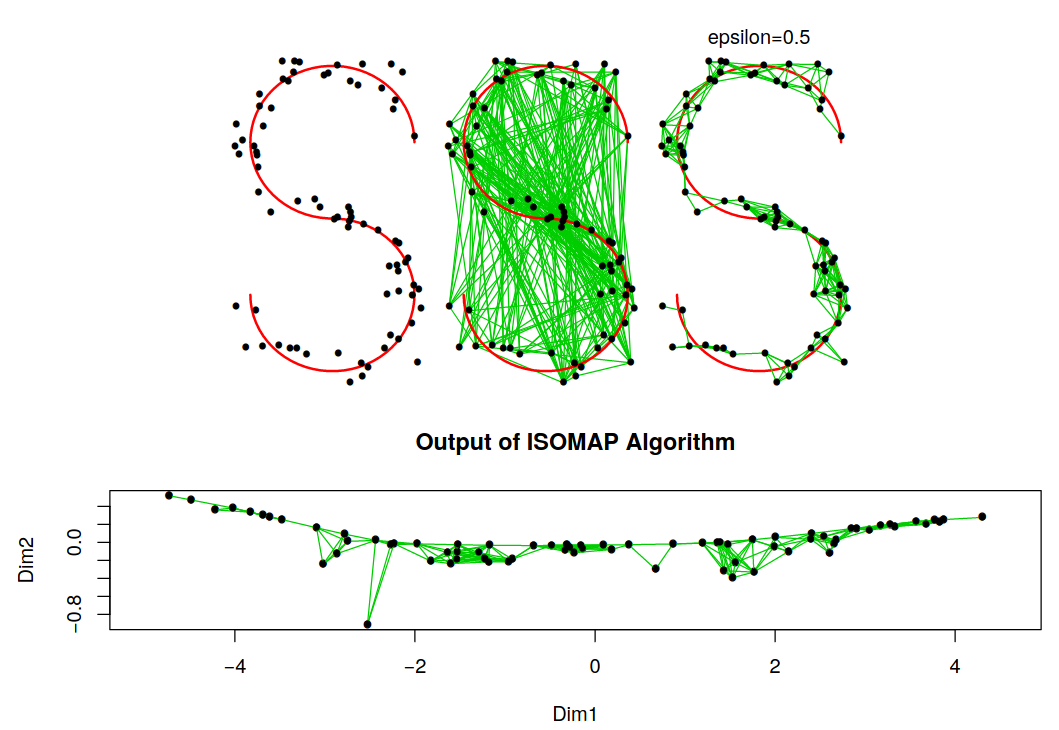
\includegraphics{isomap}
	\caption{Output of the ISOMAP algorithm.}
\end{figure}

\subsection{Role of the bandwidth parameter}
ISOMAP only depends on a tuning parameter $\varepsilon$ or $k$ that is used to
define the neighbourhood relations.

\begin{marker}
    The result if \emph{very} sensible to the \emph{bandwidth} value and can result
	in short-circuits or fragmented graph $G^\varepsilon$.
\end{marker}

There are several methods to select the bandwidth parameter, but there
is no consensus on which one is the best.

\pagebreak
\section[t-Stochastic Neighbor Embedding]{t-Stochastic Neighbor Embedding (t-SNE)}
\sectionmark{t-SNE}

\subsection{Stochastic Neighbor Embedding (SNE)}
It is an alternative to Local MDS or ISOMAP.

SNE requires a distance matrix $\boldsymbol D$ of size $n \times n$ with
entries $\delta_{ij} \geq 0$, the dissimilarity (or distance) between
individuals $i$ and $j$.

Alternatively, starting from a data matrix $\boldsymbol X$ of size $n \times p$,
(with $p$ variables and $n$ individuals), one can compute the pairwise
Euclidean distances $\boldsymbol D$: $\delta_{ij} = \lVert \boldsymbol x_i - \boldsymbol x_j \rVert$.

SNE starts by converting the high-dimensional distances between data points
into conditional probabilities $p_{i \mid j}$ that represent similarities:
\begin{equation*}
	p_{i \mid j} =
	\begin{cases}
		\frac{\exp(-\delta_{ij}^2 / 2\sigma_i^2)}{\sum_{k \neq i} \exp(-\delta_{ik}^2 / 2\sigma_i^2)} & \text{if } i \neq j \\
		0                                                                                             & \text{if } i = j
	\end{cases}
\end{equation*}
where $\sigma_i$ is a data-point dependent \iemph{bandwidth} parameter.

\begin{note}
	$p_{i \mid j}$ is the probability that a point $\boldsymbol x_i$ would pick
	point $\boldsymbol x_j$ as its neighbour if neighbours were picked in proportion
	to their probability density under a Gaussian centered at $\boldsymbol x_i$.
\end{note}

For the low-dimensional counterparts $\boldsymbol y_i$ and $\boldsymbol y_j$ of
the high-dimensional points $\boldsymbol x_i$ and $\boldsymbol x_j$, a similar
conditional probability is computed:
\begin{equation*}
	q_{i \mid j} =
	\begin{cases}
		\frac{\exp(-\lVert \boldsymbol y_i - \boldsymbol y_j \rVert^2)}{\sum_{k \neq i} \exp(-\lVert \boldsymbol y_k - \boldsymbol y_i \rVert^2)} & \text{if } i \neq j \\
		0                                                                                                                                         & \text{if } i = j
	\end{cases}
\end{equation*}
In this case, the same bandwidth $\frac{1}{\sqrt{2}}$ is used for every $\boldsymbol y_i$.

This way, every point $\boldsymbol y_i$ in the low-dimensional configuration will be
equally densely surrounded by its neighbours, leading to a better visualization.

If the low-dimensional points $\boldsymbol y_i$ and $\boldsymbol y_j$ correctly model
the similarity between the high-dimensional data points $\boldsymbol x_i$ and $\boldsymbol x_j$,
then the conditional probabilities $p_{i \mid j}$ and $q_{i \mid j}$ will be equal.

\begin{marker}
	SNE aims to find a low-dimensional data representation that minimizes
	the mismatch between the conditional probabilities $p_{i \mid j}$ and $q_{i \mid j}$.
\end{marker}

\begin{definition}{Kullback-Leibler divergence}
	The Kullback-Leibler divergence between two probability distributions $p$ and $q$ is defined as:
	\begin{equation*}
		KL(p \mid\mid q) = \sum_{j} p_j \log \frac{p_j}{q_j}
	\end{equation*}
	\tcblower
	\begin{note}
        Kullback-Leibler divergence is \emph{not symmetric}: there is a large
		cost for using widely separated map points $\boldsymbol y_i$ to
		represent nearby data points $\boldsymbol x_j$, but there is only a small
		cost for using nearby map points to represent widely separated data points.
	\end{note}
\end{definition}

\begin{problem}{Stochastic Neighbor Embedding (SNE)}{}

SNE minimizes (in a gradient descent fashion) the sum of Kullback-Leibler
divergences between the conditional distributions over all data points:
\begin{equation*}
	C(\boldsymbol Y) = \sum_{i=1}^n KL(P_i \mid\mid Q_i) =
	\mathlarger{\sum_{i=1}^n} \sum_{j=1}^n p_{i \mid j} \log \frac{p_{i \mid j}}{q_{i \mid j}}
\end{equation*}
\tcblower
\begin{note}
    The SNE cost function focuses on retaining the \emph{local structure} of the data in
	the map.
\end{note}
\end{problem}

\subsubsection{Choosing $\sigma_i$}

\begin{definition}{Shannon entropy}{}
	The Shannon entropy of a probability distribution $P$ is defined as:
	\begin{equation*}
		H(P) = - \sum_{j} p_j \log_2 p_j
	\end{equation*}
\end{definition}

\begin{definition}{Perplexity}{}
	The perplexity of a probability distribution $P$ is defined as:
	\begin{equation*}
		\text{Perp}(P) = 2^{H(P)}
	\end{equation*}
	\tcblower
	We can interpret it as the number of possible points in a uniform
	distribution having the same Shannon entropy as $P$.
	\tcbline
	\begin{note}
		When applied to the conditional distribution $P_i = \{p_{j\mid i}\}^n_{j=1}$,
		the perplexity is a measure of the number of neighbours that each point has.
	\end{note}

\end{definition}

\begin{marker}
	SNE performs a binary search to find the $\sigma_i$ that produces a
	$P_i$ with the desired perplexity (specified by the user).
\end{marker}

This method is fairly robust and typical values for the desired perplexity
range from 5 to 50.

\subsubsection{Symmetric cost function}
In order to improve the gradient descent, we can use a modified cost function
that is symmetric:
\begin{align*}
	q_{ij}           & = \frac{\exp(-\lVert \boldsymbol y_i - \boldsymbol y_j \rVert^2)}{\sum_{k \neq i} \exp(-\lVert \boldsymbol y_k - \boldsymbol y_i \rVert^2)} \\
	p_{ij}           & = \frac{p_{i \mid j} + p_{j \mid i}}{2n}                                                                                                    \\
	C(\boldsymbol Y) & =
	\mathlarger{\sum_{i=1}^n} \sum_{j=1}^n p_{ij} \log \frac{p_{ij}}{q_{ij}}
\end{align*}

\subsubsection{The crowding problem of SNE}
If the intrinsic dimension of the observed object is moderate (say 10),
the standard 2-dimensional dimensionality reduction, performed for
visualization, can not give good results. Since pairwise distances
in a 2-dimensional space cannot faithfully model distances between points
on the 10-dimensional manifold, the resulting map will be very \iemph{crowded}.

\begin{marker}
	In practice, the consequence of the crowding problem is that many
	high-dimensional points that are at moderate distance from the
	center of the data, are crushed together in the center of the
	low-dimensional map, which prevents gaps from forming between the
	natural clusters.
\end{marker}

The crowding problem is not specific to SNE, it also affects other
dimensionality reduction techniques such as non-classical metric MDS,
Local MDS or ISOMAP.

To solve this problem, we need to use t-SNE instead.

\subsection{t-Stochastic Neighbor Embedding (t-SNE)}

The main change in t-SNE with respect to SNE is the way the joint
probabilities $q_{i \mid j}$ for $i \neq j$ are computed:
\begin{equation*}
	q_{i \mid j} = \frac
	{
		(1 + \lVert \boldsymbol y_i - \boldsymbol y_j \rVert^2)^{-1}
	}{
		\sum_{k \neq i} (1 + \lVert \boldsymbol y_k - \boldsymbol y_i \rVert^2)^{-1}
	}
\end{equation*}
That is, a Student's t-distribution with 1 degree of freedom (A Cauchy distribution)
is used to transform the distances in the low dimensionality.

Additionally, t-SNE uses the symmetric version of the cost function.

\subsubsection{Software}
\begin{itemize}
	\item \texttt{tsne} fully implemented in R.
	\item \texttt{Rtsne} R interface to the a C++ implementation of t-SNE.
\end{itemize}

% \section{t-Stochastic Neighbor Embedding}
